\documentclass[xcolor={dvipsnames}]{beamer}
\usepackage{amsmath}
% \usepackage{beamerthemesplit} // Activate for custom appearance
\usepackage{hyperref}
\usepackage{ragged2e}
\usepackage{amssymb}
\usepackage{verbatim}







\title{Statistical Hypothesis Testing}
\author{Schwartz}
\date{\today}

\begin{document}

\frame{\titlepage}

\frame
{
 \frametitle{A Brief History of Statistics (Part I)}

{
\fontfamily{<familyname>}\selectfont
\begin{quote}
\tiny
\justify

 $\textrm{\underline{Significance testing}}$ is largely the product of Karl Pearson (1857--1936), William Sealy Gosset (1876--1937), and Ronald Fisher (1890--1962), although evidence of its use dates back to Laplace (1749--1827) in the 1770's.    
Pearson created the notion of a $\textrm{\emph{p-value}}$ and (Pearson's) $\textrm{\emph{chi-squared test}}$ and founded the 
world's first statistics department at University College London in 1911.  
Gosset developed and penned the $\textrm{\emph{t-distribution}}$ and $\textrm{\emph{t-test}}$ under the 
pseudonym Student due to the objections of his employer -- the original Guinness Brewery in Dublin, Ireland -- regarding publication of internal practices.  And Fisher created $\textrm{\emph{analysis of variance}}$ and popularized the notions of $\textrm{\emph{null hypothesis}}$ and $\textrm{\emph{significance test}}$. In addition to being regarded as the father of modern statistical science and experimental design, Fisher also made significant contributions to agricultural biology and genetics.  Indeed,  Richard Dawkins named him ``the greatest biologist since Darwin". 

$\quad\quad$  $\textrm{\underline{Hypothesis testing}}$ was developed by Jerzy Neyman (1894 -- 1981) and Egon Pearson (1895--1980, son of Karl Pearson). Building on these ideas, Neyman later introduced $\textrm{\emph{confidence intervals}}$ into the statistics landscape.   At the time of the publication of their work on hypothesis testing in 1933,
Neyman and Pearson (along with Fisher) were faculty members at the University College London in the department of statistics (founded by the older Pearson).   
While Fisher as a result of his agricultural background emphasized rigorous experimental design and methods to extract a result from few samples assuming Gaussian distributions, Neyman (who teamed with the younger Pearson) emphasized mathematical rigor and methods to obtain more results from many samples and a wider range of distributions. 

$\quad\quad$ Initially a $\textrm{\emph{Bayesian}}$, Fisher but sought to provide a more ``objective'' approach to inference. The significance testing he developed did not use the notion of an alternative hypothesis -- only a null hypothesis -- and hence did not involve the notion of $\textrm{\emph{Type II error}}$. Fisher's interpretation of p-values was informal: p-values were only meant to provide guidance for potential future experiments.  Neyman and Pearson on the other hand formalized hypothesis testing with $\textrm{\emph{Type I/II errors}}$ and developed a procedure to choose between competing hypotheses. They considered their formulation to be an improved and more objective generalization of significance testing as it provided a decision making tool to determine researcher behavior without requiring any inductive inference on the part of the researcher.  

\end{quote}
}
}




\frame
{
 \frametitle{A Brief History of Statistics (Part II)}

{
\fontfamily{<familyname>}\selectfont
\begin{quote}
\tiny
\justify

Fisher and Neyman/Pearson clashed bitterly, and often --  
they all shared the same building at the University College London they had ample opportunity 
to cross paths (and swords -- although only Fisher was ever knighted -- and not until many years later -- and Neyman was, after all, Polish, not English).  
They disagreed about the proper role of models in statistical inference. 
Fisher thought the Neyman/Pearson approach was not applicable to scientific research because (1) initial assumptions about the null hypothesis are often discovered to be questionable as unexpected sources of error appear over the course of the experiment and (2) rigid reject/accept decisions based on models formulated before data is collected are incompatible with the real-world scenario faced by scientists and attempts to apply such formulations to scientific research would lead to mass confusion (as it has). 

$\quad\quad$ In 1938 Neyman left University College London and moved to the University of California, Berkeley.  
This put much of the planetary diameter between both his partnership with Pearson and his dispute with Fisher.
A further respite in the debate was provided by World War II.  Nonetheless, the disagreement between Fisher and Neyman only terminated (unresolved after 27 years) with Fisher's death in 1962.  
Neyman wrote a well-regarded eulogy of Fisher upon his death.  
And some of Neyman's later publications reported p-values and significance levels.\\${}$\\${}$\\

Afterword:${}$\\${}$\\
In an apparent effort to provide a ``non-controversial'' theory (as well as likely from confusion and misunderstanding of the topic, $\textrm{\emph{per se}}$)
the modern version of hypothesis testing used today is an inconsistent hybrid of the ``Fisher versus Neyman/Pearson'' formulations developed in the early 20th century.  Rather than comparing two directly competing realistic hypotheses, one of the hypotheses is made to be a ``no effect null hypothesis'' so (despite great conceptual differences and caveats) p-values can be interpreted from both the Fisher and the Neyman/Pearson perspectives.  Neyman and Pearson provided the stronger terminology, the more rigorous mathematics and the more consistent philosophy, but the hypothesis testing used today has more similarities with Fisher's method than theirs.

\end{quote}
}
}


\frame
{
 \frametitle{Outline}

\begin{itemize}
\item Know what a \textbf{\emph{null hypothesis}} is
\begin{itemize}
\item Know what an \textbf{\emph{$\alpha$-significance level}} is
\begin{itemize} 
\item Know what a \textbf{\emph{two-tailed versus one-tailed test}} is
\item \textcolor{gray}{Know how this relates to \textbf{\emph{confidence intervals}}}
\end{itemize}
\item Know what a \textbf{\emph{p-value}} is (don't you \emph{dare} mess this up *EVAR*)
\end{itemize}
\item \textcolor{gray}{Know what an \textbf{\emph{alternative hypothesis}} is}
\begin{itemize}
\item \textcolor{gray}{Know what \textbf{\emph{power}} is}
\end{itemize}
\item \textcolor{gray}{Know what Type I and Type II errors are}
\item And know yourself a little \emph{Bonferroni} and \emph{FDR}
\item[]

\item  \textcolor{NavyBlue}{Be able to navigate in the hypothesis testing universe: }  
\begin{itemize}
\color{NavyBlue}
\item z/t-test with common or unique variances, or paired samples
\item Pearson's $\chi^2$-test, and other $\chi^2$-tests
\item Fisher's exact test
\item The other ``usual suspects'' in terms of non-parametric tests
\item Kolmogorov-Smirnov (K-S) test
\item F-test
\item And be able to \underline{correctly apply them where appropriate}
\end{itemize}
\end{itemize}

}

\frame
{
 \frametitle{Hypothesis Testing Concepts I: \textcolor{black}{\textbf{The Scientific Method}}}


\begin{enumerate}
\item[0.] What is your \emph{question}?
\item<2-> What is your \emph{population} \textcolor{NavyBlue}{(i.e., statistical distribution)}?
\item<3-> Specify a \emph{null hypothesis $H_0$}\\
${}$\\
\textcolor{Maroon}{\underline{Null hypothesis $H_0$}\\
A  ``no effect''/``boring baseline'' statement to ``disprove''\\
\emph{E.g., proposing no difference between two population means}\\${}$\\}

\item<4-> Choose a \emph{test statistic} \textcolor{NavyBlue}{that is dependent on $H_0$}

\item<5-> Determine the statistic's \emph{theoretical distribution} \textcolor{NavyBlue}{if $H_0$ is true}

\item<6-> Specify a \textcolor{Maroon}{$H_0$ \emph{rejection region}}, i.e., values of the test statistic 
which cast great doubt \textcolor{NavyBlue}{(i.e.,  $\alpha$ level)} on the accuracy of $H_0$\\
${}$\\

\textcolor{Maroon}{
\underline{Significance level $\alpha$}
$$\alpha = \text{Pr}(\text{rejecting $H_0$} | H_0 \text{ is true}) = \text{Pr}(\text{``Type I error''})$$
}
\vspace{-.5em}
\item<7-> Collect data and \emph{compute the test statistic}

\end{enumerate}

}



\frame
{
 \frametitle{Hypothesis Testing Concepts II: \textcolor{black}{\textbf{REJECTING} $H_0$}}

 \vspace{-1em}
 
\begin{enumerate}
\item[7.] Reject $H_0$ if the test statistic \textcolor{NavyBlue}{looks ``strange''}. \textcolor{gray}{The statistic is a sample from the null distribution conditional on $H_0$ being true, so if it doesn't look right then $H_0$ seems wrong...}
\end{enumerate}
%compared to its sampling distribution under the null hypothesis; otherwise, fail to reject the null hypothesis

 \vspace{-2.75em}

 
\begin{columns}
\begin{column}{.185\textwidth}
\end{column}
\begin{column}{.615\textwidth}
  
 \begin{figure}
\centering
\hspace*{-.28em}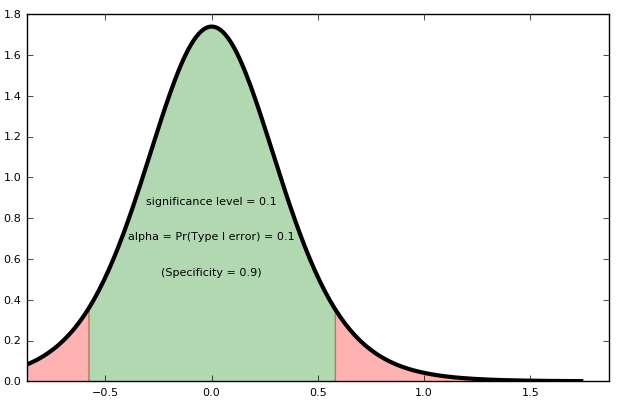
\includegraphics[width=2.73in]{stuff/tests_1.png}
\end{figure}

\vspace{-.388in}
\onslide<1->{
\color{blue}
\hspace{1.4495in}X
}
\end{column}
\begin{column}{.2\textwidth}

\onslide<1->{\textcolor{white}{Oh, and -- We \emph{NEVER ``accept''} $H_0$}}
\end{column}
\end{columns}

 \vspace{1em}

\color{white}
\onslide<1->{  \underline{p-value}\\

$\text{Pr}(\text{seeing something as or more extreme than what you saw} | H_0 \text{ true})$\\${}$\\}

\vspace{-.5em}

\onslide<1->{\underline{\emph{One-tailed} VS. \emph{two-tailed tests}}\\
How probability $\alpha$ defining a Type I error  is allotted over $H_0$ }

}



\frame
{
 \frametitle{Hypothesis Testing Concepts II: \textcolor{black}{\textbf{REJECTING} $H_0$}}

 \vspace{-1em}
 
\begin{enumerate}
\item[7.] Reject $H_0$ if the test statistic \textcolor{NavyBlue}{looks ``strange''}. \textcolor{gray}{The statistic is a sample from the null distribution conditional on $H_0$ being true, so if it doesn't look right then $H_0$ seems wrong...}
\end{enumerate}
%compared to its sampling distribution under the null hypothesis; otherwise, fail to reject the null hypothesis

 \vspace{-2.5em}

 \vspace{-.025in}
 
\begin{columns}
\begin{column}{.185\textwidth}
\end{column}
\begin{column}{.615\textwidth}
  
 \begin{figure}
\centering
\hspace*{-.4em}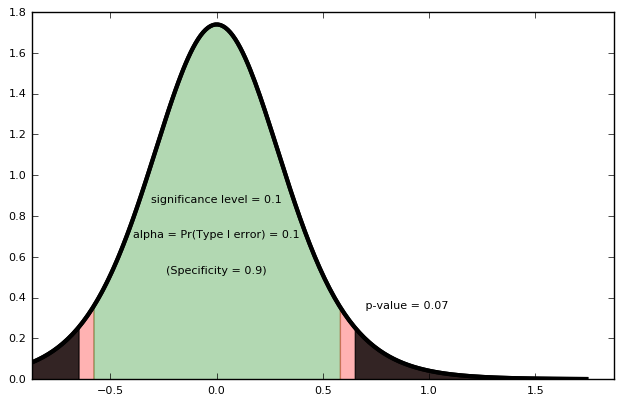
\includegraphics[width=2.75in]{stuff/tests_2.png}
\end{figure}

\vspace{-.3925in}
\onslide<1->{
\color{blue}
\hspace{1.4495in}X
}
\end{column}
\begin{column}{.2\textwidth}

\onslide<4->{\textcolor{red}{Oh, and -- We \emph{NEVER ``accept''} $H_0$}}
\end{column}
\end{columns}

 \vspace{1em}

\color{Maroon}
\onslide<2->{  \underline{p-value}\\

$\text{Pr}(\text{seeing something as or more extreme than what you saw} | H_0 \text{ true})$\\${}$\\}

\vspace{-.5em}

\onslide<3->{\underline{\emph{One-tailed} VS. \emph{two-tailed tests}}\\
How probability $\alpha$ defining a Type I error  is allotted over $H_0$ }

}





\frame
{
\frametitle{P-value \emph{blunders for which I'll never forgive you} \\\textcolor{gray}{and which will \emph{haunt} you for the \emph{rest} of your \emph{natural life}}}

\begin{itemize}
\item[X] A p-value \textcolor{red}{\underline{\emph{is not}}} the probability $H_0$ is False
\item[\checkmark] $H_0$ is True, or it is not -- there is no ''sometimes/probability''
\item[] 
\item[X]<2-> A p-value \textcolor{red}{\underline{\emph{is not}}} the probability of incorrectly rejecting $H_0$
\item[\checkmark]<2-> Significance level $\alpha$ is the probability of wrongly rejecting $H_0$
\item[]
\item[X]<3-> A p-value \textcolor{red}{\underline{\emph{is not anything else except}}} 
$\Large\text{Pr}(\textbf{seeing something as or more}$\\ 
$\Large\quad\;\;\textbf{extreme than what you saw} \;  | H_0 \text{ is true})$\\${}$\\

\item[\checkmark]<4-> A p-value is, \emph{at all times, ever only and \underline{EXACTLY ONLY}} 
$\Large\text{Pr}(\textbf{seeing something as or more}$\\ 
$\Large\quad\;\;\textbf{extreme than what you saw} \; | H_0 \text{ is true})$
\end{itemize}
}





\frame
{
 \frametitle{The \emph{Pivot} (i.e., 95\% Confidence Intervals)}

If $H_0$ is true, then 
\footnotesize
\begin{align*}
\Pr\left( -t_{n-1}^{\alpha/2} < \frac{\bar x - \mu_0} {\hat \sigma /\sqrt{n}} < t_{n-1}^{\alpha/2}\right) &=  \Pr\left( -\bar x -t_{n-1}^{\alpha/2} \frac{\hat \sigma}{\sqrt{n}} < - \mu_0 <  -\bar x  +t_{n-1}^{\alpha/2} \frac{\hat \sigma}{\sqrt{n}} \right)\\
&=  \Pr\left( \bar x +t_{n-1}^{\alpha/2} \frac{\hat \sigma}{\sqrt{n}} > \mu_0 >  \bar x  - t_{n-1}^{\alpha/2} \frac{\hat \sigma}{\sqrt{n}} \right)\\
&= \Pr\left( \bar x - t_{n-1}^{\alpha/2} \frac{\hat \sigma}{\sqrt{n}} < \mu_0 <  \bar x  + t_{n-1}^{\alpha/2} \frac{\hat \sigma}{\sqrt{n}} \right)
\end{align*}
\normalsize
``captures'' $\mu_0$ in 95\% of hypothetically repeated experiments 

\vspace{-1em}
\begin{figure}
\centering
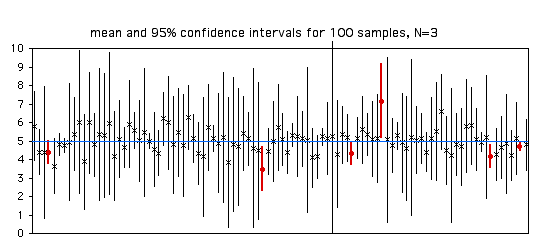
\includegraphics[width=4.25in]{stuff/conf1.png}
\end{figure}
}



\frame
{
 \frametitle{Confidence Intervals and p-values \emph{equivalence}}

\begin{figure}
\centering
\large
A $100(1-\alpha)\%$ confidence interval \emph{does not contain} $\mu_0$

\vspace{-4em}
\Huge\onslide<2->{$$\iff$$\\${}$\\}
\vspace{-1.5em}
\large

\onslide<2->{A two-sided test \emph{rejects} $H_0$ at the $\alpha$-significance level}\\${}$\\${}$\\${}$\\



\onslide<3->{A $100(1-\alpha)\%$ confidence interval \emph{contains} $\mu_0$} 

\vspace{-4em}
\Huge\onslide<4->{$$\iff$$\\${}$\\}
\vspace{-1.5em}
\large

\onslide<4->{A two-sided test \emph{fails to reject} $H_0$ at the $\alpha$-significance level}\\

\end{figure}
}

\frame
{
 \frametitle{Confidence Intervals and p-values \emph{equivalence}}

\begin{itemize}
\item[]
\textcolor{gray}{If $H_0$ is true, then 
\begin{align*}
\alpha = {} & \text{Pr}_{\bar x}\left(\left\lvert  \frac{\bar x - \mu_0} {\hat \sigma /\sqrt{n}}\right\rvert > Z_{\alpha/2} \right)
\end{align*}
\item[] The observed p-value under $H_0$ is 
\begin{align*}
p = {} & \text{Pr}_Z\left( Z > \left\lvert  \frac{\bar x - \mu_0} {\hat \sigma /\sqrt{n}}\right\rvert \right)\quad
\end{align*}
}
\item<1-> \underline{\textcolor{red}{If $p < \alpha$ then}} $\left\lvert \frac{\bar x - \mu_0} {\hat \sigma /\sqrt{n}}\right\rvert > Z_{\alpha/2} $
\item[]<1-> \textcolor{gray}{$\Longrightarrow \mu_0 < \bar x - Z_{\alpha/2} \frac{\hat \sigma}{\sqrt{n}} \text{ or } 
\mu_0 > \bar x + Z_{\alpha/2} \frac{\hat \sigma}{\sqrt{n}}$}
\item[]<2-> $\Longrightarrow \mu_0 \not \in \left(\bar x - Z_{\alpha/2} \frac{\hat \sigma}{\sqrt{n}}, 
\bar x + Z_{\alpha/2} \frac{\hat \sigma}{\sqrt{n}}\right)$
\item[] 
\item[]<2-> \textcolor{red}{\underline{i.e., the $100(1-\alpha)\%$ confidence interval \emph{does not} contain $\mu_0$}}
\end{itemize}
}




\frame
{
 \frametitle{Hypothesis Testing Concepts III}

\begin{itemize}
\item \underline{Alternative hypothesis $(H_A)$}\\
An ``actual'' hypothesized truth about a distribution on data, distinct from $H_0$'s, 
often used to characterize a tests power\\
\emph{E.g., assuming group $A$'s mean is twice that of group $B$}\\${}$\\

\item \underline{Test \emph{power} $\beta$}
\begin{align*}
\beta =& \text{Pr}(\text{Fail to rejecting $H_0$} | H_A \text{ is true})\\
=& \text{Pr}(\text{Type II error})
\end{align*}
\end{itemize}
}




\frame
{
 \frametitle{Hypothesis Testing Concepts III}
 
 \begin{figure}
\centering
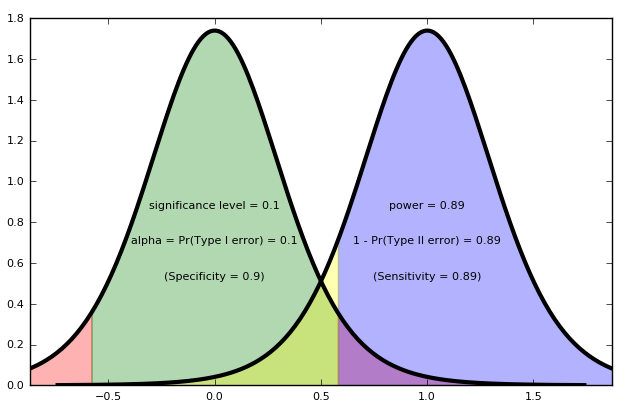
\includegraphics[width=3.5in]{stuff/tests_3.png}
\end{figure}

\textcolor{white}{
P-values are not related to relative likelihoods.
Compared to all alternatives, p-values  $\sim 0.05$
  are very strong evidence for  $H_0$.\\${}$\\ 
If some extreme  $H_A$
  is true then you'd never see anything like  $0.05$, but if  $H_0$
  is true then you would...}

}

\frame
{
 \frametitle{Hypothesis Testing Concepts III}
 
 \begin{figure}
\centering

\vspace*{.1em}
\hspace*{-.1em}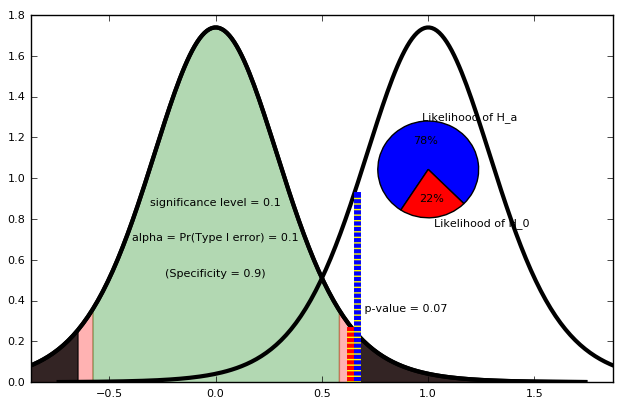
\includegraphics[width=3.5in]{stuff/tests_4.png}
\end{figure}

\onslide<2->{\textcolor{NavyBlue}{
P-values are not related to relative likelihoods.
Compared to all alternatives, p-values  $\sim 0.05$
  are very strong evidence for  $H_0$.\\${}$\\ 
If some extreme  $H_A$
  is true then you'd never see anything like  $0.05$, but if  $H_0$
  is true then you would...}}

}



\frame
{
 \frametitle{\textcolor{white}{More} Practice}

\begin{itemize}
\item Yankees fan proportion versus Mets fan proportion
\item[]
\item[]
\item[]
\item[]
\item[]
 
\item<2-> Cat weights versus Dog weights
\item[]
\item[]
\item[]
\item[]
\item[]

\end{itemize}
}



\frame
{
\frametitle{More Practice}
  
\begin{table}
\centering
\begin{tabular}{r|c|c}
&
\includegraphics[height=1in]{stuff/p6.png}&
\includegraphics[height=1in]{stuff/p2.png}\\ && \\\hline
Trial 1 & \onslide<2->{$\emptyset$} & \\ 
Trial 2 &  & \onslide<3->{$\emptyset$} \\ 
Trial 3 &  & \onslide<4->{\checkmark} \\ 
Trial 4 & \onslide<5->{$\emptyset$} &  \\ 
$\vdots$ & & \\ 
Trial $n_{\textcolor{gray}{A}} + n_{\textcolor{gray}{B}}$ & &\\  \hline 
Total & \onslide<6->{$\hat p_{\textcolor{gray}{A}} = \frac{\sum X_{\textcolor{gray}{A}}^{\textcolor{gray}{(i)}}}{n_{\textcolor{gray}{A}}}$\hspace{4em}} & \onslide<6->{$\hat p_{\textcolor{gray}{B}} = \frac{\sum X_{\textcolor{gray}{B}}^{\textcolor{gray}{(j)}}}{n_{\textcolor{gray}{B}}}}$\hspace{4em}
\end{tabular}
\end{table}
}

\frame
{
\frametitle{More Practice: A/B testing}

$$\hat p_{\textcolor{gray}{A}} = \frac{\sum X_{\textcolor{gray}{A}}^{\textcolor{gray}{(i)}}}{n_{\textcolor{gray}{A}}} \quad \quad \hat p_{\textcolor{gray}{B}} = \frac{\sum X_{\textcolor{gray}{B}}^{\textcolor{gray}{(j)}}}{n_{\textcolor{gray}{B}}}$$

\begin{align*} 
   X_{\textcolor{gray}{A}}^{\textcolor{gray}{(i)}} \sim {}& \text{Bern}\left(\theta_{\textcolor{gray}{A}}\right) \textcolor{gray}{= \text{Binomial}\left(\theta_A,N_A=1\right)} \\
   X_{\textcolor{gray}{B}}^{\textcolor{gray}{(j)}} \sim {}& \text{Bern}\left(\theta_{\textcolor{gray}{B}}\right) \textcolor{gray}{= \text{Binomial}\left(\theta_B,N_B=1\right)} \\
   \\
   {\text{\usebeamercolor[fg]{structure} IF }} {}& \theta_{\textcolor{gray}{A}} = \theta_{\textcolor{gray}{B}} \quad\quad\quad\quad\quad\quad\quad\quad\quad\;\;\; \textcolor{gray}{\text{[$H_0$]} } \\
   {\text{\usebeamercolor[fg]{structure} THEN }} {}& Var\left(X_{\textcolor{gray}{A}}^{\textcolor{gray}{(i)}}\right) = Var\left(X_{\textcolor{gray}{B}}^{\textcolor{gray}{(j)}}\right) = \;\textcolor{gray}{?} \\ 
   {\text{\usebeamercolor[fg]{structure} SO } } {}& \hat p_{\textcolor{gray}{A}} - \hat p_{\textcolor{gray}{B}} \sim \; \textcolor{gray}{? \quad\quad\quad\quad\quad\quad\quad\quad \text{[By CLT]} } \\
   \textcolor{gray}{\text{AND } } {}&  \textcolor{gray}{\text{what is a good estimator of } \theta = \theta_A = \theta_B? } \\
\end{align*}
}

% E[b] = E[B] = p = 1-q
% Var(b) = Var(B) = pq
% Var(sum(b)/n) = 1/n^2 sum(b) = 1/n^2 n(pq) = pq/n
% Var(sum(b)/n - sum(B)/m) = pq/n + pq/m


\frame
{
\frametitle{Multiple Testing}

\vspace{-.75em}

\begin{columns}
\begin{column}{1\textwidth}
\hspace*{-1em}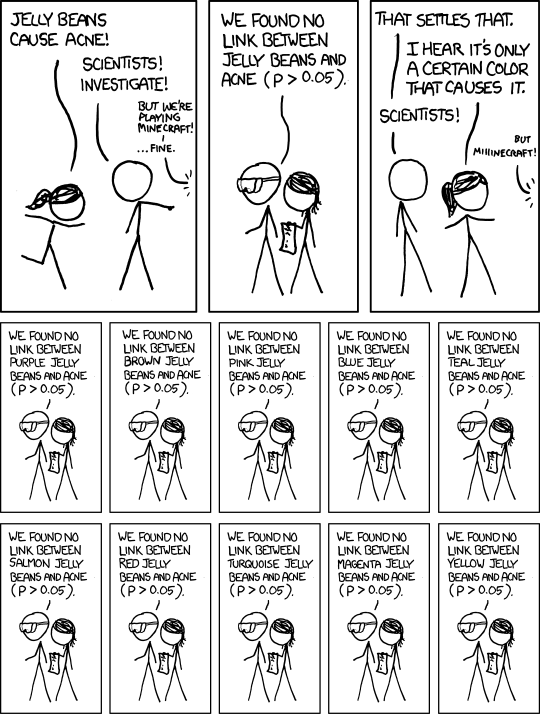
\includegraphics[width=2.25in]{stuff/significant1.png}$\quad$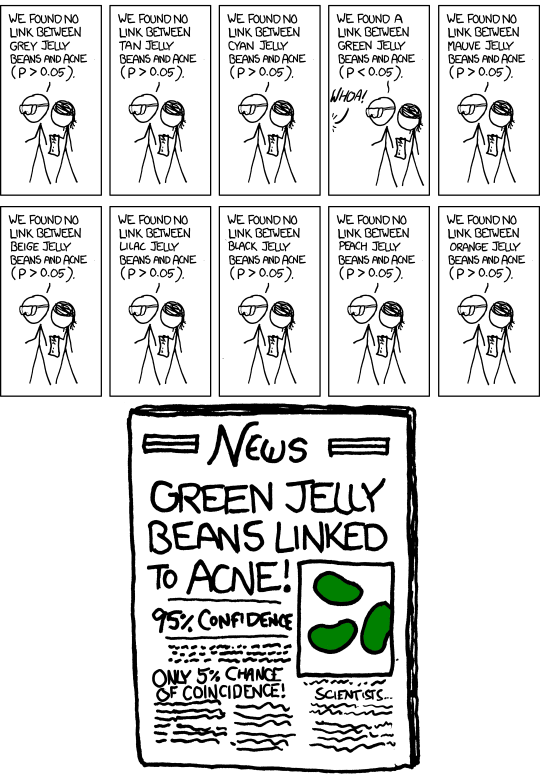
\includegraphics[width=2.09in]{stuff/significant2.png}
\end{column}
\end{columns}


}


\frame
{
\frametitle{Multiple Testing}

\begin{itemize}
\item Each time we do a hypothesis test \textcolor{gray}{[what?]}
\item[]<2-> There's a chance we are wrong about our decision
\item<3-> If $H_0$ is true, an $\alpha$ chance of being wrong
\item[]<4-> So if we do $N$ tests, and $H_0$ is true for all of them
\item[]<5-> \emph{we still expect to wrongly reject $H_0$ about $\alpha \times N$ times!}
\item<6-> Testing at $\alpha' = \alpha/N$ gives an $\alpha$ chance all tests are right
\item<7-> This is called \emph{Bonferroni correction} 
\item[]<8-> and it guarantees a $\alpha$ \emph{familly-wise error rate} 
\item[]
\item<9-> Bonferroni correction is really quite stringent... 
\item[]
\item<10-> An alternative is the \emph{False Discovery Rate (FDR)} $q$
\item[]<11-> which for a set of tests (e.g., tests significant at the $\alpha$-level)
\item[]<12-> is the proportion $q$ of the tests called incorrectly (``FDR")
\end{itemize}

}


\frame{
\frametitle{\textbf{Multiple} A/B Testing}

\begin{itemize}%[leftmargin=*]
\item There is no difference in conversion rates in these simulations
\end{itemize}

\vspace{-2em}
\setlength{\leftmargini}{-30pt}
\begin{itemize}%[leftmargin=*]
\item[] 
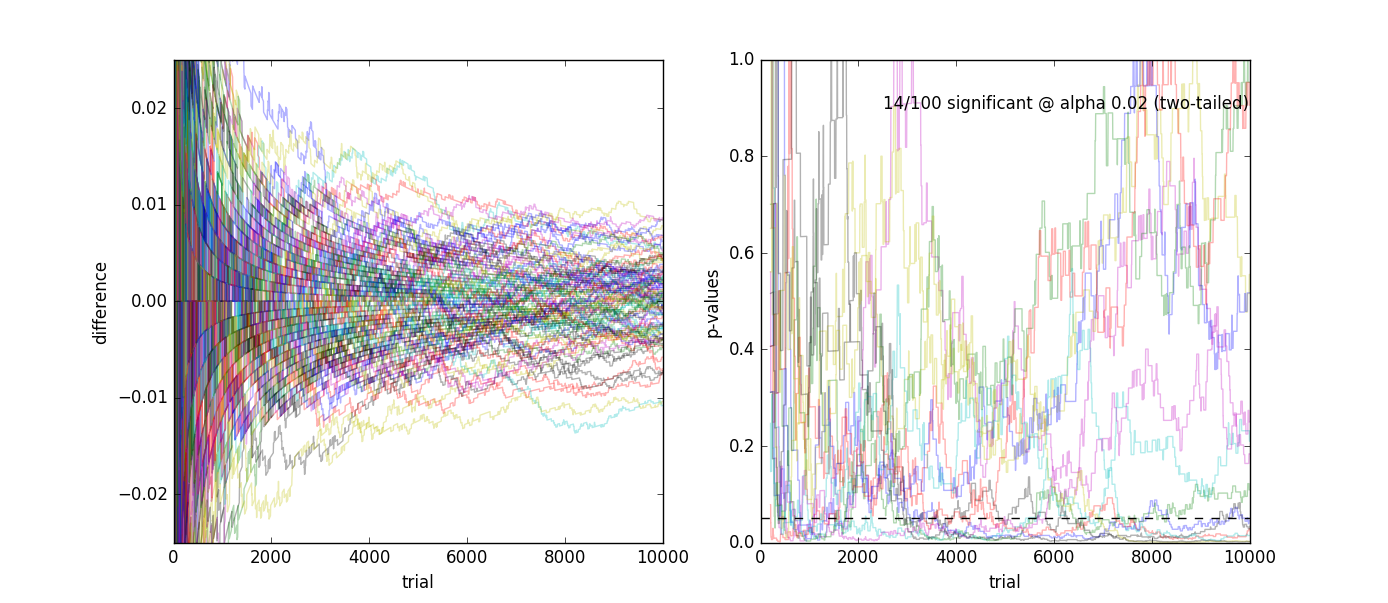
\includegraphics[height=2.25in]{stuff/figure_1.png}
\end{itemize}

\vspace{-.5em}
\setlength{\leftmargini}{25pt}
\begin{itemize}%[leftmargin=*]
\item<1> Continuous (multiple) testing does not achieve $\alpha$-significance
\end{itemize}

}






\end{document}

\frame{
\frametitle{A/B \textbf{Hypothesis Testing} \emph{significance}}
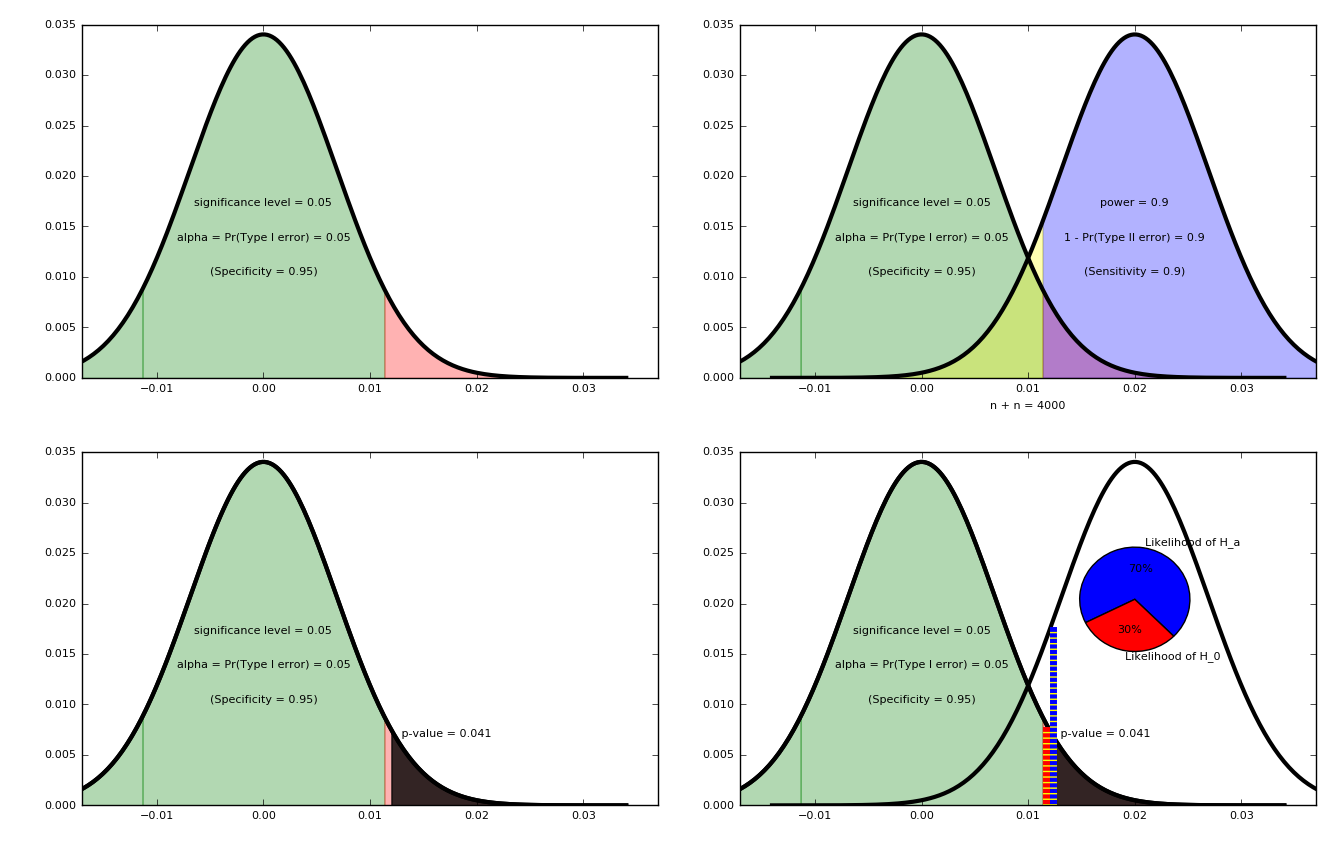
\includegraphics[width=4.25in]{pvals.png}
}



\frame
{
\frametitle{A/B \textbf{Hypothesis Testing} \emph{questions}}
\begin{itemize}

\footnotesize
\item[] Suppose we think a new site is better than an old site
\item<2-> What's the $\alpha$ significance level we're testing at?
\item<3> How do we get it? 
\item<4-> We observed a very small p-value, $p$...  what's the...
\item[]<4-7> probability the new site is better than the old site (i.e. $H_0$ false)?
\item[]<5-7> probability both sites are the same (i.e. $H_0$ true)?
\item[]<6-7> probability that we correctly concluded the new is better than the old?
\item[]<7> probability that we incorrectly concluded the new is better than the old?
\item<8-12> Can we say there's a  
\item[]<8-12> $100\cdot(1-p)$\% chance the new site is better?
\item[]<9-12> $100\cdot p$\% chance that both sites are the same?
\item[]<10-12> $100\cdot(1-\alpha)$\% chance the new site is better?
\item[]<11-12> $100\cdot\alpha$\% chance that both sites are the same?
\item[]<12> $100\cdot\alpha$\% chance that we incorrectly concluded the sites are different?
\end{itemize}
}



\frame
{
 \frametitle{Hypothesis Testing}
 
 \begin{figure}
\centering
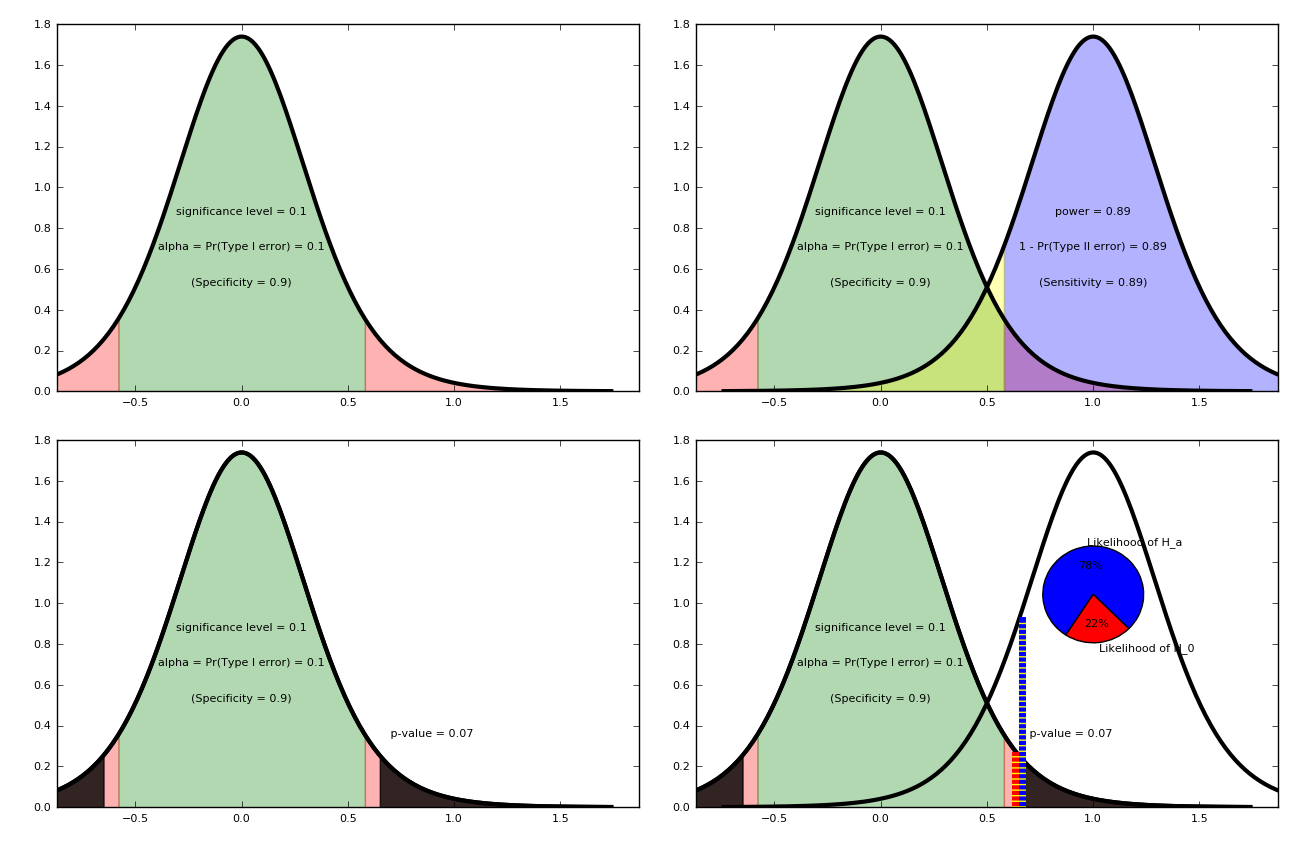
\includegraphics[width=4in]{tests.png}
\end{figure}
\vspace{-1.5em}
\begin{itemize}
\item<2> What $\alpha$ significance level are we testing at?
\vspace{-1.5em}
\item<3> How did we choose this $\alpha$ significance level?
\vspace{-1.5em}
\item<4> How did we construct this $\alpha$ significance level?
\vspace{-1.5em}
\item<5> We observed a p-value of 0.07... what's $\Pr(H_0 \text{ True})$?
\vspace{-1.5em}
\item<6> We observed a p-value of 0.07... what's $\Pr(H_0 \text{ False})$?
\vspace{-1.5em}
\item<7> We observed a p-value of 0.07... $\Pr(H_0 \text{ Incorrectly Rejected})$?
\vspace{-2.75em}
\item<8> We observed a p-value of 0.07... $\Pr(H_0 \text{ Correctly Accepted})$?
\vspace{-1.5em}
\item<9> $\alpha = 0.1$.... is there a 90\% chance $H_a$ is True?
\vspace{-1.5em}
\item<10> $\alpha = 0.1$.... is there a 10\% chance $H_0$ is False?
\vspace{-1.5em}
\item<11> $\alpha = 0.1$.... is there a 10\% chance $H_a$ is True?
\vspace{-1.5em}
\item<12> $p = 0.07$... is there a 93\% chance $H_0$ is True?
\vspace{-1.5em}
\item<13> $p = 0.07$... is there a 7\% chance $H_0$ is False?
\vspace{-1.5em}
\item<14> $p = 0.07$... is there a 7\% chance $H_a$ is True?
\vspace{-1.5em}
\item<15> $p = 0.07$...  does $\Pr(H_0 \text{ Incorrectly Rejected}) = 0.07$?
\vspace{-1.5em}
\item<16> $p = 0.07$...  does $\Pr(H_0 \text{ Correctly Accepted}) = 0.93$?
\vspace{-1.5em}
\item<17>  What is $\Pr(H_0 \text{ Incorrectly Rejected})$?
\vspace{-1.5em}
\item<18>  What is $\Pr(H_0 \text{ Rejected } | \; H_0 \text{ True})$?
\vspace{-1.5em}
\item<19> What is $\Pr(H_0 \text{ Correctly Rejected})$?
\vspace{-1.5em}
\item<20> What is $\Pr(H_0 \text{ Rejected } | \; H_a \text{ True})$?
\vspace{-1.5em}
\item<21>  What is $\Pr(H_0 \text{ Accepted } | \; H_0 \text{ True})$?
\vspace{-1.5em}
\item<22> What is $\Pr(H_0 \text{ Accepted } | \; H_a \text{ True})$?
\end{itemize}
}



\frame
{
\frametitle{Parametric Versus Nonparametric}

We might characterize an analysis framework as parametric if

\begin{enumerate}
\item Results are buttressed or bolstered by modeling assumptions 
\textcolor{gray}{\emph{E.g., leveraging the structure of normality via a t-test increases power but comes at a cost of 
loss of robustness compared to 
nonparametric tests free of distributional assumptions. 
}}
\item Predicted values are based on ``parameters.'' \\
\textcolor{gray}{\emph{E.g., the $\beta$ coefficients in linear regression.}}
\item Parameter estimation  
determines the specific instance of a model within a ``model class'' defined by those parameters. \\
\textcolor{gray}{\emph{E.g., the CLT is based on a normal distribution which is determined by estimating $\mu$ and $\sigma^2.$}}
\item The complexity of the model does grows as data size $n$ grows.
\textcolor{gray}{\emph{E.g., trees grow in complexity as data becomes richer while a normal distribution is defined by $\mu$ and $\sigma^2$ regardless of $n$.}}
\end{enumerate}
}










\begin{frame}[fragile]
\frametitle{Single Sample Test Class}

\begin{verbatim}
from scipy import stats

print xbar, mu_0, se, n
# 1, 0, 0.5, 30

2*(1-stats.t.cdf(loc = (xbar - mu_0)/se, df = n-1))


\end{verbatim}

Let's make this into a class!

\end{frame}



\begin{frame}[fragile]
\frametitle{Single Sample Test Class}
\begin{verbatim}
from scipy import stats

print xbar, mu_0, se, n
# 1, 0, 0.5, 30

stats.t.cdf(loc = (xbar - mu_0)/se, df = n-1))
\end{verbatim}
\end{frame}





